\chapter{Argomenti: la spugna di Menger}
{ }\hfill\textbf{Livello:} Avanzato \\

In questo capitolo costruiremo un solido frattale chiamato spugna di Menger. Questi sono i primi passi per creare questo solito:

\begin{center}
	\begin{minipage}{6cm}
		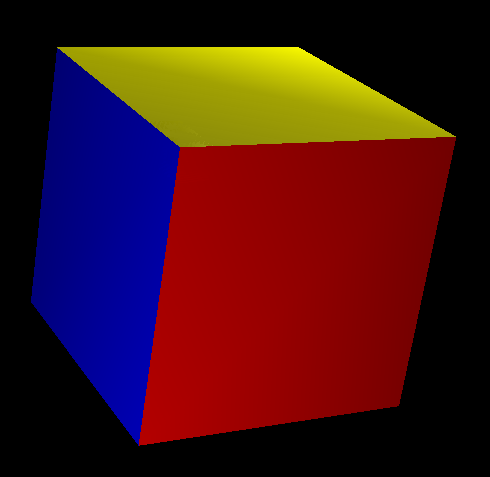
\includegraphics[width=6cm]{pics/menger0.png}
		\begin{center}
			\textbf{Passo 0}
		\end{center}
	\end{minipage}
	\begin{minipage}{6cm}
		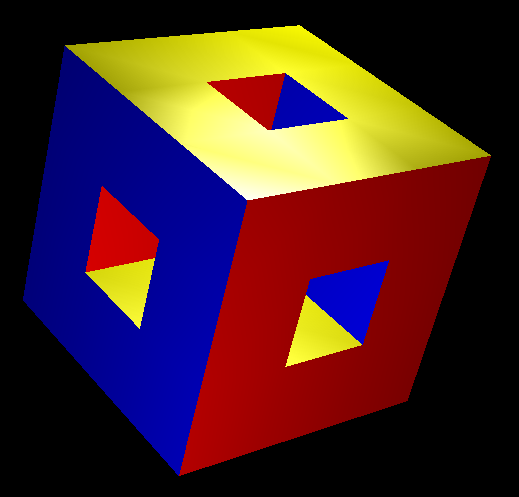
\includegraphics[width=6cm]{pics/menger1.png}
		\begin{center}
			\textbf{Passo 1}
		\end{center}
	\end{minipage}
\\
	\begin{minipage}{6cm}
		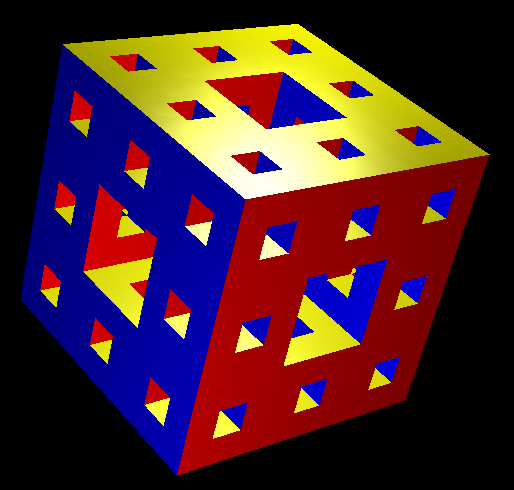
\includegraphics[width=6cm]{pics/menger2.png}
		\begin{center}
			\textbf{Passo 2}
		\end{center}
	\end{minipage}
	\begin{minipage}{6cm}
		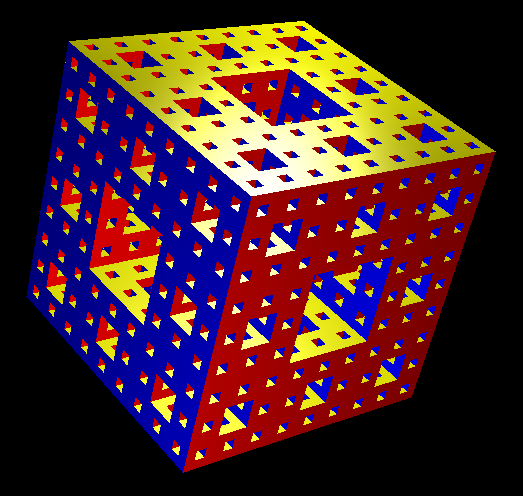
\includegraphics[width=6cm]{pics/menger3.png}
		\begin{center}
			\textbf{Passo 3}
		\end{center}
	\end{minipage}
\end{center}

Questo capitolo contiene due sezioni:
\begin{itemize}
	\item Per primo vedremo come creare questo solido utilizzando la ricorsione.
	\item Infine proveremo a generare una spugna di Menger di ordine~4.
\end{itemize}



\section{Primo approccio: ricorsione}
Consideriamo una spugna di Menger di ordine $n$ con spigolo $L$.\\
\begin{center}
	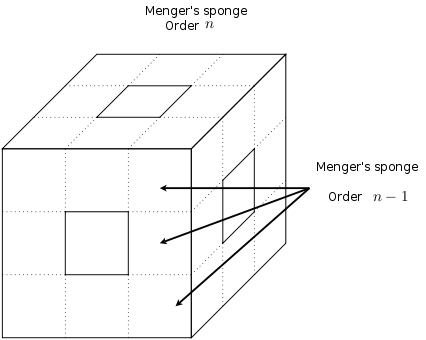
\includegraphics{pics/menger-schema01.png}
\end{center}

Nello schema notiamo che la spugna contiene 20 spugne di Menger di ordine $n-1$ di spigolo $\dfrac{L}{3}$. La natura ricorsiva della spugna e' evidente.\\

\subsection{Il programma}

\begin{lstlisting}[frame=single]
per cubo :l
	Se :counter=10000 [VistaPoligono3D]
	AssegnaVarLocale "colori [Giallo Magenta Ciano Blu]
	# facce laterali
	Ripeti 4 [ImpostaColorePenna Lancia Elemento ContaRipetizioni :colori 
	quadrato :l RuotaDestra 90 Avanti  :l RuotaSinistra 90 RollioDestra 90]
	# faccia inferiore
	ImpostaColorePenna Rosso BeccheggiaGiu 90 quadrato :l BeccheggiaSu 90
	Avanti :l BeccheggiaGiu 90 ImpostaColorePenna Verde quadrato :l 
	BeccheggiaSu 90 Indietro :l
fine

per quadrato :c
	AssegnaVar "counter :counter+1
	InizioPoligono
	Ripeti 4 [Avanti :c RuotaDestra 90]
	FinePoligono
fine

# spugna di menger
# p: ordine di ricorsione
# l: spigolo del cubo
per menger :l :p
	Se :p=0 [cubo :l] [
	  AssegnaVarLocale "p :p-1  
	  AssegnaVarLocale "l :l/3
	  # faccia frontale
	  Ripeti 3 [menger :l :p Avanti :l] Indietro 3*:l
	  RuotaDestra 90 Avanti :l RuotaSinistra 90
	  menger :l :p Avanti 2*:l menger :l :p Indietro 2*:l
	  RuotaDestra 90 Avanti :l RuotaSinistra 90
	  Ripeti 3 [menger :l :p Avanti :l] Indietro 3*:l
	  # faccia di destra
	 BeccheggiaGiu 90 Avanti :l BeccheggiaSu 90 
	  menger :l :p  Avanti 2*:l menger :l :p Indietro 2*:l
	  BeccheggiaGiu 90 Avanti :l BeccheggiaSu 90 
	  Ripeti 3 [menger :l :p Avanti :l] Indietro 3*:l
	  RuotaSinistra 90 Avanti :l RuotaDestra 90
	  menger :l :p  Avanti 2*:l menger :l :p Indietro 2*:l
	  RuotaSinistra 90 Avanti :l RuotaDestra 90
	  Ripeti 3 [menger :l :p Avanti :l] Indietro 3*:l
	  BeccheggiaGiu 90 Indietro :l BeccheggiaSu 90
	  menger :l :p  Avanti 2*:l menger :l :p Indietro 2*:l
	   BeccheggiaGiu 90 Indietro :l BeccheggiaSu 90
	]
fine

per spugna :p
	PulisciSchermo NascondiTartaruga AssegnaVar "counter 0 3D 
	ImpostaColoreSfondo 0 menger 800 :p 
	Scrivi [nombre ColorePenna polygone: ] Stampa :counter 
	VistaPoligono3D
fine
\end{lstlisting}

Il programma ha quattro procedure:
\begin{itemize}
 \item \texttt{quadrato :c}\\
Questa procedura disegna un quadrato di lato \texttt{:c}. Il poligono viene immagazzinado nel visualizzatore 3D. La variabile \texttt{counter} conta il numero dei poligoni disegnati.
 \item \texttt{cubo :l}\\
La procedura disegna un cubo di spigolo \texttt{:l}. Ovviamente utilizza \texttt{quadrato}.
 \item \texttt{menger :l :p}\\
Questa e' la procedura più importante, disegna le linee di Menger di ordine $p$ di lunghezza $l$. La linea e' creata usando la ricorsione come abbiamo visto nello schema.
 \item \texttt{spugna :p}\\
Questa procedura crea la spugna di Menger, di ordine $p$ con spigolo pari a 800 e la disegna nel visualizzatore 3D.
\end{itemize}
\vfill
Il vantaggio di questo programma e' di sfruttare la struttura ricorsiva del solido. Il metodo e' molto simile a quello usato per disegnare il fiocco di neve di Van Kock a pagina \pageref{vankoch}. Il vantaggio della ricorsione e' una codice piuttosto snello.\\
Il principale svantaggio di questo approccio e' che, essendo ricorsivo, richiede molta memoria per la sua esecuzione. Infatti una spugna di ordine 3 disegna 48000 poligoni. \xlogo\ richiede in questo caso di alzare il limite della memoria interna di 256 MB (impostabile nel pannello delle preferenze) per prevenire l'overflow.



\section{Secondo approccio: il tappeto Sierpinski}
Se vogliamo disegnare una spugna di Menger di ordine 4, dobbiamo ripensare il programma e dimenticare la ricorsione. Creeremo un programma che disegnerà il solido di Menger di ordine 0, 1, 2, 3 e 4.

\subsection{il tappeto di Sierpinski}
La spugna di Menger e' una generalizzazione in 3 dimensioni di una figura piana chiamata ``tappeto di Sierpinski''. Questi sono i primi passi per generare questa figura:

\begin{minipage}{4.5cm}
	\begin{center}
		
\includegraphics[width=4.5cm]{pics/carpet0.png}\\
		\textbf{Passo 0}
	\end{center}
\end{minipage}
\begin{minipage}{4.5cm}
	\begin{center}
		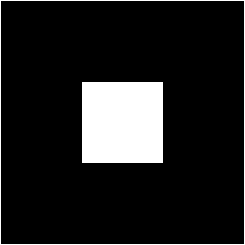
\includegraphics[width=4.5cm]{pics/carpet1.png}\\
		\textbf{Passo 1}
	\end{center}
\end{minipage}
\begin{minipage}{4.5cm}
	\begin{center}
		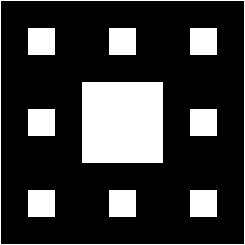
\includegraphics[width=4.5cm]{pics/carpet2.png}\\
		\textbf{Passo 2}
	\end{center}
\end{minipage}
\begin{minipage}{4.5cm}
	\begin{center}
		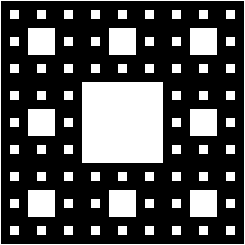
\includegraphics[width=4.5cm]{pics/carpet3.png}\\
		\textbf{Passo 3}
	\end{center}
\end{minipage}\\ 
\vspace*{0.5cm}\\

Ciascuna faccia della spugna di Menger di ordine $p$ e' un tappeto di Sierpinski di ordine $p$.


\subsection{Disegnare un tappeto Sierpinski di ordine $p$}
L'obiettivo e' di usare il minor numero possibile di poligoni per disegnare un tappeto Sierpinski. Il seguente esempio spiega come disegnare un tappeto di ordine 3. Il primo quadrato ha $3^3=27$ linee e 27 colonne. Scriviamo in base 3 ciascun numero di riga e ciascun numero di colonna.
\begin{itemize}
	\item [\textbullet]\textbf{Primo passo}: Per ciascuna riga il cui numero non cintiene alcun 1, disegniamo una riga di 27 unità. Usando la simmetria ripetiamo la stessa operazione sulle colonne.\\
	\begin{center}
		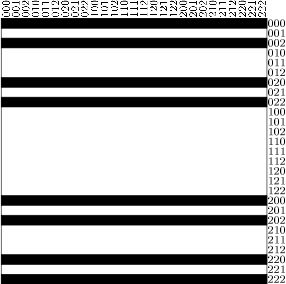
\includegraphics{pics/menger-schema02.png}
		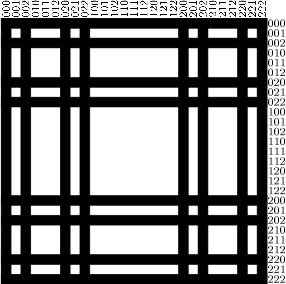
\includegraphics{pics/menger-schema03.png}
	\end{center}
	\vspace{0.2cm}
	\item [\textbullet] \textbf{Secondo passo}: Adesso guardiamo alle righe i cui numeri hanno un singolo 1 al primo posto. Disegniamo rettangoli di 9 unità di lunghezza in modo alternato.
	\begin{center}
		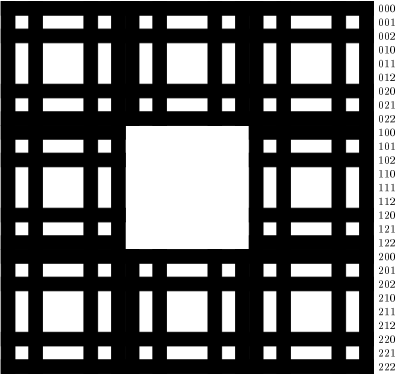
\includegraphics{pics/menger-schema04.png}
	\end{center} 
	\item [\textbullet] \textbf{Terzo passo}: Adesso consideriamo le righe il cui numero contiene un singolo 1 al secondo posto. Disegniamo rettangoli seguendo lo schema $[3\ 3\ 6\ 3\ 6\ 3\ 3]$ (cioe' 3 unità penna giù, 3 unità penna sù, 6 unità penna giù \textellipsis). Usando la simmetria ripetiamo l'operazione sulle colonne.
	\begin{center}
		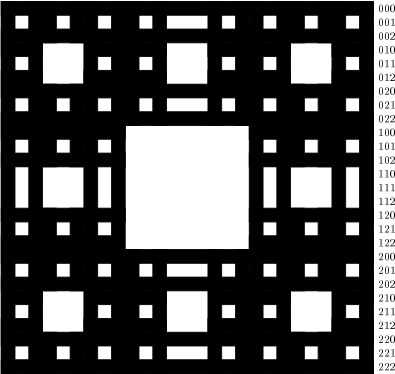
\includegraphics{pics/menger-schema05.png}
	\end{center}
	\item [\textbullet] \textbf{Passo finale}: Consideriamo le righe il cui numero contiene un 1 due volte nelle prime due posizioni. Disegniamo rettangoli alternati seguendo lo schema $[3\ 3\ 3\ 9\ 3\ 3\ 3]$. Ripetiamo lo stesso sulle colonne.
	\begin{center}
		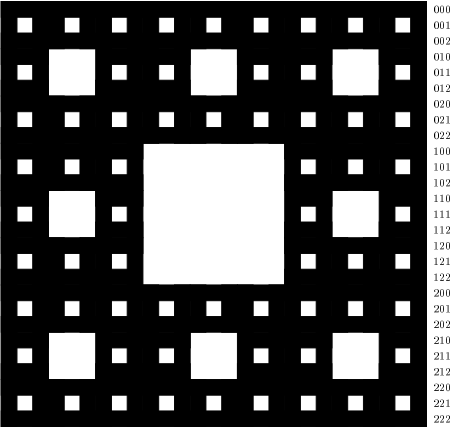
\includegraphics{pics/menger-schema06.png}
	\end{center}
\end{itemize}
Abbiamo costruito un tappeto Sierpinski di ordine 3. Per disegnare tale poligono abbiamo bisogno di $16+16+32+16=80$ poligoni.



\subsection{Tutti i diversi possibili schemi per le colonne}
Per riassumere, ecco i diversi schemi delle colonne per i vari numeri di riga (il simbolo * rappresenta 0 o 2).
\begin{center}
	\begin{tabular}{|c|c|}
		\hline
		Numero di righe & Schema da applicare\\
		\hline
		*** & 27 \\ 
		\hline
		1** &  9 9 9 \\
		\hline
		*1* & 3 3 6 3 6 3 3\\
		\hline
		11* & 3 3 3 9 3 3 3\\
		\hline
	\end{tabular}
\end{center}

Allo stesso modo, per costruire un tappeto di ordine 4 abbiamo bisogno di un quadrato di $3^4=81$ unità. Le righe e le colonne avranno numeri a base 3 di 4 cifre. Per ciascun numero di riga ecco lo schema da applicare (il simbolo * rappresenta 0 o 2).
\begin{center}
	\begin{tabular}{|c|c|}
		\hline
		Numero di righe & Schema da applicare\\
		\hline
		**** & 81 \\ 
		\hline
		1*** &  27 27 27 \\
		\hline
		*1** & 9 9 18 9 18 9 9 \\
		\hline
		**1* & 3 3 6 3 6 3 6 3 6 3 6 3 6 3 6 3 6 3 3 \\
		\hline
		*11* &  3 3 3 9 3 3 6 3 3 9 3 3 6 3 3 9 3 3 3 \\
		\hline
		1*1* & 3 3 6 3 6 3 3 27 3 3 6 3 6 3 3 \\
		\hline
		11** & 9 9 9 27 9 9 9 \\
		\hline
		111*& 3 3 3 9 3 3 3 27 3 3 3 9 3 3 3 \\
		\hline
	\end{tabular}\\
\end{center}
496 poligoni sono necessari in questo caso.\\
Infine questo e' lo schema per una figura di ordine 2.
\begin{center}
	\begin{tabular}{|c|c|}
		\hline
		Numero di righe & Schema da applicare\\
		\hline
		** &  9 \\
		\hline
		1* & 3 3 3 \\ 
		\hline
	\end{tabular}
\end{center}


\subsection{Il programma}
\begin{lstlisting}[frame=single]
# disegna un tappeto sierpinski carpet di ordine :p e dimensione :size
per carpet :size :p
	AssegnaVar "unit :size/(Potenza 3 :p)
	Se :p=0 [ rec :size :size Ferma]
	Se :p=1 [Ripeti 4 [rec :size :unit Avanti :size RuotaDestra 90 ] Ferma]
	RipetiPer (Elenco "x 1 Potenza 3 :p) [
	  AssegnaVarLocale "cantorx cantor :x :p []
	# non abbiamo disegnato gli elementi con un 1 in Ultimo Posizione
	Se  non (1=last :cantorx)  [
	  AssegnaVarLocale "nom evalue EccettoUltimo :cantorx "
	  drawcolumn :x Proprieta "map :nom
	  ]
	]  
fine

# Restituisce il numero in base 3
# p ordeine del tappeto
# :list Elenco vuoto
per cantor :x :p :list
	Se :p=0 [Output :list] 
	AssegnaVarLocale "a Potenza 3 :p-1
	Se :x<= :a [
	  Output cantor  :x :p-1  Frase :list 0] 
	  [ Se :x<=2*:a [Output cantor  :x-:a :p-1  Frase :list 1] 
	  Output cantor :x-2*:a :p-1 Frase :list 0]
fine

# Disegna la colonna numero x
# rispetto lo schema nell'elenco :list
per drawcolumn :x :list
	PennaSu  RuotaDestra 90 Avanti (:x-1)*:unit RuotaSinistra 90  
	PennaGiu des :list
	PennaSu RuotaSinistra 90 Avanti (:x-1)*:unit RuotaDestra 90 
	Avanti :x*:unit RuotaDestra 90 PennaGiu des :list
	PennaSu RuotaSinistra 90 Indietro :x*:unit PennaGiu
fine

# Disegna un rettangolo delle dimensioni scelte
# e lo immagazzina nel visualizzatore 3D
per rec :lo :la
	AssegnaVar "compteur :compteur+1
	InizioPoligono
	Ripeti 2 [Avanti :lo RuotaDestra 90 Avanti :la RuotaDestra 90]
	FinePoligono
fine

# definisce le diverse possibile colonne
per initmap
	AggiungiProprieta "map 111 [3 3 3 9 3 3 3 27 3 3 3 9 3 3 3]
	AggiungiProprieta "map 110 [9 9 9 27 9 9 9]
	AggiungiProprieta "map 101 [3 3 6 3 6 3 3 27 3 3 6 3 6 3 3]
	AggiungiProprieta "map 011 [3 3 3 9 3 3 6 3 3 9 3 3 6 3 3 9 3 3 3]
	AggiungiProprieta "map 000 [81]
	AggiungiProprieta "map 100 [27 27 27]
	AggiungiProprieta "map 010 [9 9 18 9 18 9 9]
	AggiungiProprieta "map 001 [3 3 6 3 6 3 6 3 6 3 6 3 6 3 6 3 6 3 3]
	AggiungiProprieta "map 01 [3 3 6 3 6 3 3]
	AggiungiProprieta "map 00 [27]
	AggiungiProprieta "map 10 [9 9 9]
	AggiungiProprieta "map 11 [3 3 3 9 3 3 3]
	AggiungiProprieta "map 1 [3 3 3]
	AggiungiProprieta "map 0 [9]
fine

# Se il numero in base 3 e' [1 0 1] restituisce  101
per evalue :list :mot
	Se Vuoto? :list [Output :mot]
	[
	  AssegnaVarLocale "mot Parola :mot Primo :list
	  Output evalue EccettoPrimo :list :mot  
	]
fine
	
# Disegna il blocco dei rettangoli alternati
per des :list
	AssegnaVarLocale "somme 0
	RipetiPer (Elenco "i 1 Conta :list) [
	   AssegnaVarLocale "element Elemento :i :list
	    AssegnaVarLocale "somme :element+:somme 
		  Se pari? :i [PennaSu Avanti :element*:unit PennaGiu ]
		 [rec :element*:unit :unit Avanti :element*:unit]  
	]
	PennaSu Indietro  :somme * :unit PennaGiu
fine

# :i e' un numero pari?
per pari? :i
	Output 0=resto :i 2
fine

# Disegna il tappeto di ordine :p
per tappeto :p
	PulisciSchermo 3D NascondiTartaruga initmap
	AssegnaVar "compteur 0
	carpet 810 :p
	Scrivi "Numero di poligoni:\  Stampa :compteur 
	VistaPoligono3D
fine
\end{lstlisting}

\texttt{tappeto 3} disegna un tappeto di Sierpinski di ordine 3 e di lato uguale a 810. Eccoci! Ora possiamo tornare alla spugna di Menger!


\subsection{La spugna di Menger di ordine 4}
La spugna di Menger ha molte simmetrie. Per costruire la spugna disegneremo le diverse sezioni lungo il piano $(xOy)$ e quindi ripetiamo queste figure lungo i piani $(yOz)$ e $(xOz)$. Per spiegare cosa succede consideriamo la spugna di ordine 2. Quando tagliamo con un piano verticale possiamo ottenere quattro linee:\\

\begin{center}
	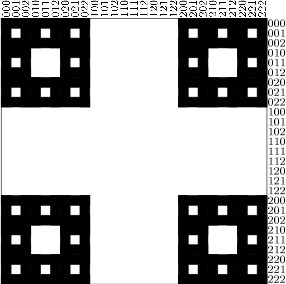
\includegraphics{pics/menger-schema07.png} \\ \vspace{1cm}
	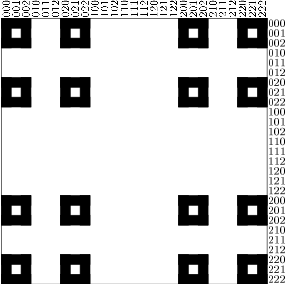
\includegraphics{pics/menger-schema08.png} \\ \vfill
	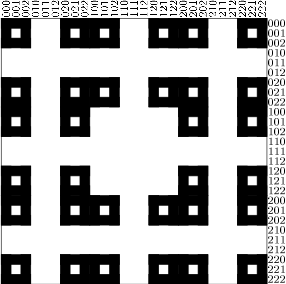
\includegraphics{pics/menger-schema09.png} \\ \vspace{1cm}
	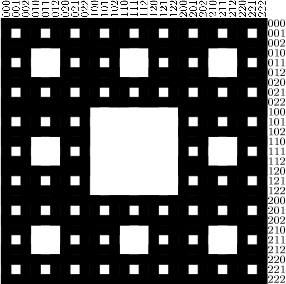
\includegraphics{pics/menger-schema10.png}\\ 
\end{center}

Per disegnare una spugna di ordine 3 faremo una ricerca nei numeri da 1 a 27, cioe' da 001 a 222 in base 3. Per ciascun numero applicheremo la sezione valida e riporteremo questa figura lungo $(Ox)$, $(Oy)$ e $(Oz)$.


\subsubsection{Il programma}
Con questo programma possiamo disegnare la spugna di Menger di ordine 0,1,2,3 e 4.

\begin{lstlisting}[frame=single]
# disegna un tappeto sierpinski carpet di ordine :p e dimensione :size
per carpet :size :p
	AssegnaVar "unit :size/(Potenza 3 :p)
	Se :p=0 [ rec :size :size Ferma]
	Se :p=1 [Ripeti 4 [rec :size :unit Avanti :size RuotaDestra 90 ] Ferma]
	RipetiPer (Lista "x 1 Potenza 3 :p) [
	  AssegnaVarLocale "cantorx cantor :x :p []
		# non abbiamo disegnato gli elementi con un 1 in Ultimo Posizione
	Se  non (1=last :cantorx)  [
	  AssegnaVarLocale "nom evalue EccettoUltimo :cantorx "
	  drawcolumn :x Proprieta "map :nom
	  ]
	]  
fine

# Restituisce il numero in base 3
# p ordeine del tappeto
# :list Elenco vuoto
per cantor :x :p :list
	Se :p=0 [Output :list] 
	AssegnaVarLocale "a Potenza 3 :p-1
	Se :x<= :a [
	  Output cantor  :x :p-1  Frase :list 0] 
	  [ Se :x<=2*:a [Output cantor  :x-:a :p-1  Frase :list 1] 
	  Output cantor :x-2*:a :p-1 Frase :list 2]
fine

# Disegna la colonna numero x
# rispetto lo schema nell'elenco :list
per drawcolumn :x :list
	PennaSu  RuotaDestra 90 Avanti (:x-1)*:unit 
	RuotaSinistra 90  PennaGiu des :list
	PennaSu RuotaSinistra 90 Avanti (:x-1)*:unit 
	RuotaDestra 90 Avanti :x*:unit RuotaDestra 90 PennaGiu des :list
	PennaSu RuotaSinistra 90 Indietro :x*:unit PennaGiu
fine

# Disegna un rettangolo delle dimensioni scelte
# e lo immagazzina nel visualizzatore 3D
per rec :lo :la
	AssegnaVar "counter :counter+1
	InizioPoligono
	Ripeti 2 [Avanti :lo RuotaDestra 90 Avanti :la RuotaDestra 90]
	FinePoligono
fine

# definisce le diverse possibile colonne
per initmap
	AggiungiProprieta "map 111 [3 3 3 9 3 3 3 27 3 3 3 9 3 3 3]
	AggiungiProprieta "map 110 [9 9 9 27 9 9 9]
	AggiungiProprieta "map 101 [3 3 6 3 6 3 3 27 3 3 6 3 6 3 3]
	AggiungiProprieta "map 011 [3 3 3 9 3 3 6 3 3 9 3 3 6 3 3 9 3 3 3]
	AggiungiProprieta "map 000 [81]
	AggiungiProprieta "map 100 [27 27 27]
	AggiungiProprieta "map 010 [9 9 18 9 18 9 9]
	AggiungiProprieta "map 001 [3 3 6 3 6 3 6 3 6 3 6 3 6 3 6 3 6 3 3]
	AggiungiProprieta "map 01 [3 3 6 3 6 3 3]
	AggiungiProprieta "map 00 [27]
	AggiungiProprieta "map 10 [9 9 9]
	AggiungiProprieta "map 11 [3 3 3 9 3 3 3]
	AggiungiProprieta "map 1 [3 3 3]
	AggiungiProprieta "map 0 [9]
fine

# Se il numero in base 3 e' [1 0 1] restituisce 101
# Se il numero in base 3 e' [1 0 2] restituisce 100
# gli elementi da :list sono tradotti in un parola
# 2 sono sostituiti da 0

per evalue :list :mot
	Se Vuoto? :list [Output :mot]
	  [
	  AssegnaVarLocale "first Primo :list
	  Se :first=2 [AssegnaVarLocale "first 0] 
	 AssegnaVarLocale "mot Parola :mot :first
	  Output evalue EccettoUltimo :list :mot  
	]
fine

# Disegna il blocco dei rettangoli alternati
per des :list
	AssegnaVarLocale "somme 0
	RipetiPer (Lista "i 1 Conta :list) [
	   AssegnaVarLocale "element Elemento :i :list
	    AssegnaVarLocale "somme :element+:somme 
	  Se even? :i [PennaSu Avanti :element*:unit PennaGiu ] 
	      [rec :element*:unit :unit Avanti :element*:unit]  
	]
	PennaSu Indietro  :somme * :unit PennaGiu
fine

# Disegna il tappeto di ordine :p
per tapis :p
	PulisciSchermo 3D NascondiTartaruga initmap
	AssegnaVar "compteur 0
	carpet 810 :p
	Scrivi "nombre\ de\ polygones:\  Stampa :compteur 
	VistaPoligono3D
fine

# :i e' un numero pari?
per even? :i
	Output 0=modulo :i 2
fine


# Rimuovi l'ultimo 1 da :list
per deletelastone :list
	RipetiPer (Lista "i Conta :list 1 Meno 1) [
	  AssegnaVarLocale "element Elemento :i :list 
	  Se :element=1 [AssegnaVarLocale "list Sostituisci :list :i 0 
	Ferma] [Se :element=2 [Ferma]]
	]
	Output :list
fine

# disegna il tappeto di serpinski 
# lungo l'asse (ox), (oy) e (oz)
per DisegnaTappeto3 :size :order :z
	PennaSu Origine  
	BeccheggiaSu 90 Avanti (:z-1)*:unite BeccheggiaGiu 90 PennaGiu
	ImpostaColorePenna Blu Lancia :order :size
	PennaSu Origine  
	RollioSinistra 90 Avanti (:z-1)*:unite BeccheggiaGiu 90  PennaGiu
	ImpostaColorePenna Giallo Lancia :order :size
	PennaSu Origine  
	BeccheggiaSu 90 Avanti :size RuotaDestra 90 Avanti (:z-1)*:unite 
	BeccheggiaGiu 90 PennaGiu
	ImpostaColorePenna Magenta Lancia :order :size 
fine

# spugna di menger di ordine :p e dimensione :size
per menger :size :p
	AssegnaVar "unite :size/(Potenza 3 :p)
	RipetiPer (Lista "z 1 Potenza 3 :p) [
	  AssegnaVarLocale "cantorz cantor :z :p []
	  AssegnaVarLocale "last Ultimo :cantorz
	  AssegnaVarLocale "cantorz EccettoUltimo :cantorz
	  Se :last=0 [AssegnaVarLocale "order evalue deletelastone :cantorz "] 
	           [AssegnaVarLocale "order evalue :cantorz "]
	  AssegnaVarLocale "order Parola "coupe :order
	  DisegnaTappeto3 :size :order :z
	  PennaSu BeccheggiaSu 90 Avanti :unit BeccheggiaGiu 90 PennaGiu 
	]
	DisegnaTappeto3 :size :order (Potenza 3 :p)+1
fine


# procedure pricipale
# disegna una spugna di ordine :p di spigolo 405
per sponge :p
	PulisciSchermo ImpostaColoreSfondo 0 3D NascondiTartaruga
	AssegnaVarLocale "time SecondiDaAvvio
	initmap
	AssegnaVar "counter 0
	Se :p=0 [cube 405] [menger 405 :p]
	# Visualizza il tempo di esecuzione
	Scrivi "numero\ poligoni:\  Stampa :counter 
	Scrivi "Tempo:\  Stampa SecondiDaAvvio -:time 
	VistaPoligono3D
fine

# diverse sezioni per menger di ordine 2
per coupe1 :size
	Ripeti 4 [carpet :size/3 1 PennaSu Avanti :size RuotaDestra 90 PennaGiu]
fine

per coupe0 :size
	carpet :size 2
fine

# diverse sezioni per menger di ordine 3

per coupe10 :size
	Ripeti 4 [carpet :size/3 2 PennaSu Avanti :size RuotaDestra 90 PennaGiu]
fine

per coupe01 :size
	Ripeti 4 [Ripeti 2 [coupe1 :size/3 PennaSu Avanti :size/3 PennaGiu] 
	Avanti :size/3 RuotaDestra 90]
fine

per coupe11 :size
	Ripeti 4 [coupe1 :size/3 PennaSu Avanti :size RuotaDestra 90 PennaGiu]
fine


per coupe00 :size
	carpet :size 3
fine

# diverse sezioni per menger di ordine 4
per coupe000 :size
	carpet :size 4
fine

per coupe100 :size
	Ripeti 4 [carpet :size/3 3 PennaSu Avanti :size RuotaDestra 90 PennaGiu]
fine

per coupe010 :size
	Ripeti 4 [Ripeti 2 [coupe10 :size/3 PennaSu Avanti :size/3 PennaGiu] 
	Avanti :size/3 RuotaDestra 90]
fine

per coupe001 :size
	Ripeti 4 [Ripeti 2 [coupe01 :size/3 PennaSu Avanti :size/3 PennaGiu] 
	Avanti :size/3 RuotaDestra 90]
fine

per coupe110 :size
	Ripeti 4 [coupe10 :size/3 PennaSu Avanti :size PennaGiu RuotaDestra 90 ]
fine

per coupe111 :size
	Ripeti 4 [coupe11 :size/3 PennaSu Avanti :size RuotaDestra 90 PennaGiu]
fine

per coupe101 :size
	Ripeti 4 [coupe01 :size/3 PennaSu Avanti :size RuotaDestra 90 PennaGiu]
fine

per coupe011 :size
	Ripeti 4 [Ripeti 2 [coupe11 :size/3 PennaSu Avanti :size/3 PennaGiu] 
	Avanti :size/3 RuotaDestra 90]
fine

per coupe :size
	carpet :size 1
fine

per cube :size
	Ripeti 2 [
	ImpostaColorePenna Blu rec :size :size PennaSu Avanti :size 
	BeccheggiaGiu 90 PennaGiu 
	ImpostaColorePenna Giallo rec :size :size PennaSu Avanti :size 
	BeccheggiaGiu 90  PennaGiu
	]
	ImpostaColorePenna Magenta
	PennaSu RollioSinistra 90 RuotaSinistra 90 Avanti :size 
	RuotaDestra 90 PennaGiu rec :size :size
	PennaSu RuotaDestra 90 Avanti :size RuotaSinistra 90 
	RollioDestra 90 RuotaDestra 90 Avanti :size RuotaSinistra 90 
	RollioDestra 90 PennaGiu rec :size  :size
	RollioSinistra 90 RuotaSinistra 90 Avanti :size RuotaDestra 90
fine
\end{lstlisting}

Occorre impostare la memoria disponibile per \xlogo\ a 640 MB: \texttt{spugna 4}.

\begin{center}
 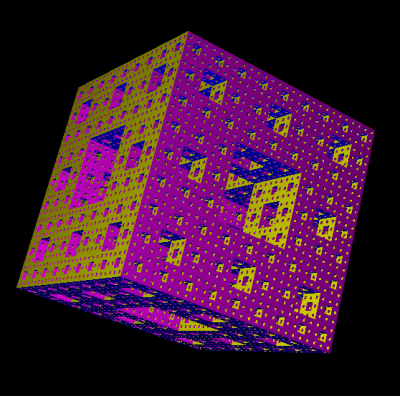
\includegraphics{pics/menger-menger4.png}
\end{center}